\documentclass{ctexart}
\usepackage{graphicx}



\title{密码学原理与实践实验报告(认证服务系统)}
\author{韦昆杰\\1181000420}

\date{\today}


\graphicspath{{images/}}

\begin{document}

\maketitle

\tableofcontents
\section{背景与意义}
\subsection{项目开发意义}
数字证书认证机构(英语:Certificate Authority,缩写为CA),也称为电子商务认证中心、电子商务认证授权机构,是负责发放和管理数字证书的权威机构,并作为电子商务交易中受信任的第三方,承担公钥体系中公钥的合法性检验的责任。所有通过CA的信息传输方,都要无条件的信任CA的公正性,在消息传输的过程中,CA为信息传输的双方提供公私钥加密环境,提供身份认证、安全传输、不可否认性和数据完整性等功能。

公钥基础设施PKI(英语:Public Key Infrastructure,缩写:PKI),是一组由硬件、软件、参与者、管理政策与流程组成的基础架构,其目的在于创造、管理、分配、使用、存储以及撤销数字证书。PKI技术采用证书管理公钥, 通过第三方的可信任机构—认证中心CA(Certificate Authority),把用户的公钥和用户的其他标识信息(如名称、E-mail、身份证号等)捆绑在一起,在Internet上验证用户的身份(其中认证机构CA是PKI系统的核心部分)。目前, 通用的办法是采用建立在PKI基础之上的数字证书,通过把要传输的数字信息进行加密和签名,保证信息传输的机密性、真实性、完整性和不可否认性,从而保证信息的安全传输。
\subsection{国内外现状及技术综述}
美国的PKI建设过程经历了1996年之前的无序、1996—2002年间以FBCA为核心的体系搭建、2003之后策略管理和体系建设并举的三个阶段。1996年以前,很多政府部门自建PKI系统,例如美国邮政服务部门、社会安全部门、美国国防部、能源部、美国商标与知识产权局等。1996年美国提出联邦桥接计划,2001年正式公布,计划最终建立一个覆盖美国80个机构、19个部的PKI以保护电子政府的通信安全。

美国联邦PKI体系主要由联邦的桥认证机构(Federal Bridge CA,FBCA)、首级认证机构(Principal CA,PCA)和次级认证机构(Subordinate CA,SCA)等组成。联邦PKI的体系结构中没有采用根CA,而采用了首级CA。

这是因为在美国,信任域的结构是多种多样的,美国联邦PKI体系结构可以支持分级(树状)维构、网状结构和信任列表等。联邦的桥CA是联邦PKI体系中能核心组织,是不同信任域之间能桥梁,主要负责为不同信任域能首级CA颁发交叉认证的证书,建立各个信任域的担保等级与联邦CA的担保等级之间的映射关系,更新交叉认证证书,发布交叉认证证书注销黑名单。但是联邦的桥CA不要求一个机构在与另一个机构发生信任关系时必须述循联邦PKI所确定的这种映射关系,而是可以采用它认为合适的映射关系确定彼此之间的信任。

欧洲在PKI基础建设方面也成绩显著。已颁布了93/1999EC法规,强调技术中立、隐私权保护、国内与国外相互认证以及无歧视等原则。为了解决各国PKI之间的协同工作问题,它采取了一系列措施:积极资助相关研究所、大学和企业研究PKI相关技术;资助PKI互操作性相关技术研究,并建立CA网络及其顶级CA。并于2000年10月成立了欧洲桥CA指导委员会,于2001年3月23日成立了欧洲桥CA。

我国的PKI技术从1998年开始起步,政府和各有关部门对PKI产业的发展给予了高度重视。2001年PKI技术被列为“十五”863计划信息安全主题重大项目,并于同年10月成立了国家863计划信息安全基础设施研究中心。国家电子政务工程中明确提出了要构建PKI体系。我国已全面推动PKI技术研究与应用。2004年8月28日,十届全国人大常委会第十一次会议28日表决通过了电子签名法,规定电子签名与手写签名或者盖章具有同等的法律效力。这部法律的诞生极大地推动了我国的PKI建设。

1998年国内第一家以实体形式运营的上海CA中心(SHECA)成立,此后,PKI技术在我国的商业银行、政府采购以及网上购物中得到了广泛应用。国内的CA机构大致可分为区域型、行业型、商业型和企业型四类,并出现了得安科技、创原世纪、国创科技、吉大正元、国瑞数码等一批PKI服务提供商。
\section{需求分析}
\subsection{总体需求}
设计实现一个认证服务系统,在消息传输的过程中,CA为信息传输的双方提供公私钥加密环境,提供身份认证、安全传输、不可否认性和数据完整性等功能。

\subsection{功能需求}
\begin{itemize}
    \item 接收验证用户数字证书的申请
    \item 生成证书
    \item 存储证书
    \item 向申请者颁发(或拒绝颁发)数字证书
    \item 接收用户数字证书的查询、撤销
    \item 产生和发布证书的有效期
    \item 数字证书的归档
    \item 密钥归档
\end{itemize}

\subsection{性能需求}
技术栈:reactjs+material-ui+mysql

本实验选用react作为前端框架,react通过引入虚拟DOM的方式显著减少了每次更新UI所进行的DOM操作,提高了效率。

通过采用客户端渲染(Client-side Rendering),相较服务器渲染(Server-side Rendering)每次都要向服务器请求HTML页面性能显著提升。

最后,每次前端向后端api接口请求数据,并根据请求数据的结果更新DOM,实现了前后端分离的同时也避免了不必要的页面更新。
\section{概要设计}
围绕着需求分析,将展开如下设计:
\subsection{接收验证用户数字证书的申请}
\begin{enumerate}
    \item 用户首先登录CA认证系统(无账号需要先注册)
    \item 用户进入申请证书页面,输入域名、国家、省份、城市、组织、组织单位等信息,在“1年”、“2年”、“3年”中选择一项作为证书的有效期,点击提交按钮。
    \item 后台处理用户的申请证书信息,将这些信息归档后,生成证书供用户下载。
    \item 用户下载证书到本地
\end{enumerate}
\subsection{生成证书}
后端根据用户申请证书输入的信息生成相应证书
\subsection{存储证书}
后端生成证书后将证书序列号、开始时间、截至时间、证书、公私钥、证书对应用户存储在数据库中(私钥用AES加密后存储)
\subsection{向申请者颁发(或拒绝颁发)数字证书}
如果申请者为已经注册证书的域名申请证书,会拒绝颁发,否则向申请者颁发数字证书
\subsection{接收用户数字证书的查询、撤销}
\begin{itemize}
    \item 查询:用户进入下载证书页面,输入需要查询的证书序列号,后台会查找数据库寻找到相应证书供用户下载
    \item 撤销:用户进入撤销证书页面,输入需要撤销的证书序列号和登录密码,如果用户是证书所有者后台会查找数据库寻找到相应证书并且撤销,否则拒绝请求。
\end{itemize}
\subsection{产生和发布证书的有效期}
证书的有效期为从证书制作时间起,1年/2年/3年止,时限由用户在申请证书时选择。
\subsection{数字证书的归档}
数字证书的归档一律以文件的形式存储在本地路径中,同时详细信息以字段形式保存在数据库中。
\subsection{密钥归档}
密钥的归档一律以文件的形式存储在本地路径中,同时密钥以字段形式保存在数据库中(公钥直接保存,私钥用用户输入口令的AES加密后保存)。


\section{详细设计}
\subsection{主页面}



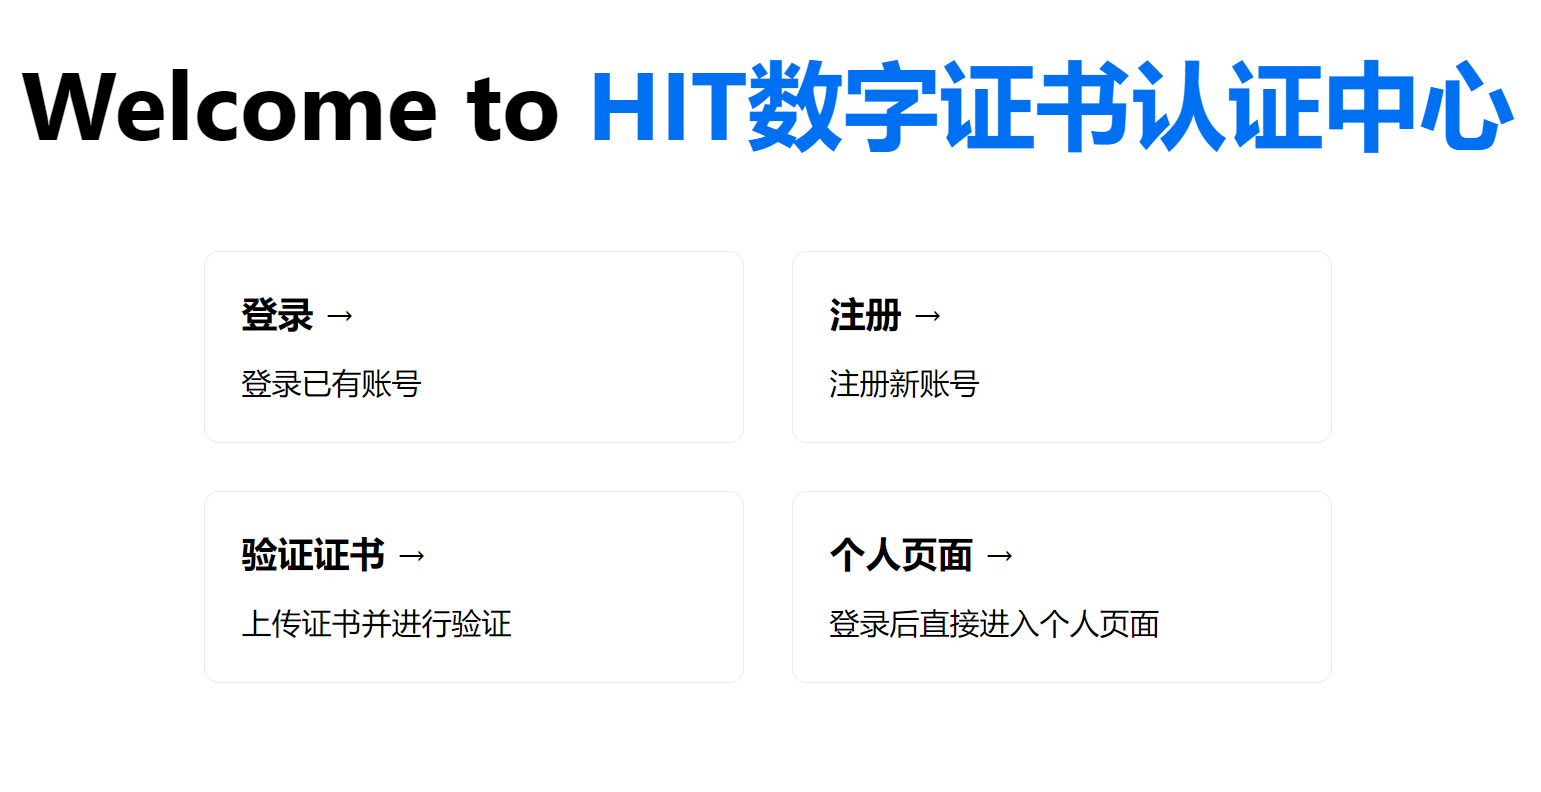
\includegraphics[width=\textwidth]{main_page.png}



网站的主页面,用户可以选择登录、注册、验证证书或进入个人页面
\subsection{注册页面}



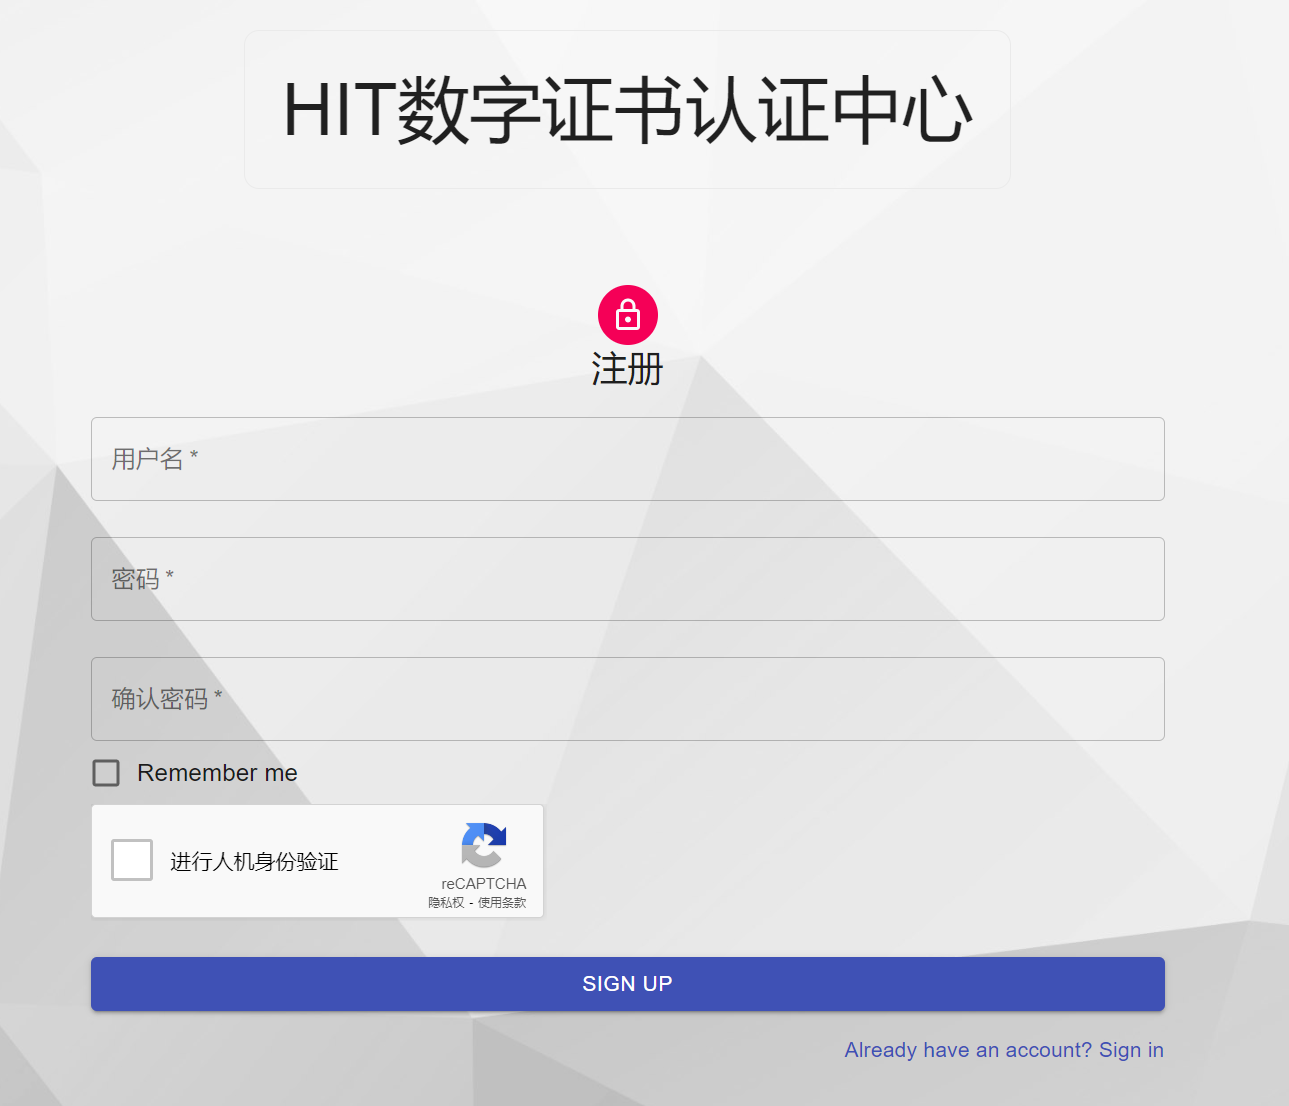
\includegraphics[ width=0.7\textwidth]{register_page.png}



用户注册需要输入用户名和密码,需要满足以下几个条件:
\begin{itemize}
    \item 用户名必须为字母、数字、下划线、减号的组合,长度为6~16位
    \item 密码至少包括数字和字母,长度至少为6位,至多20位。
\end{itemize}
最后用户还需要确认密码以及进行人机身份验证,一切无误后点击注册按钮即可成功注册,相关信息(密码用bcrypt哈希)会存入到数据库的user表中


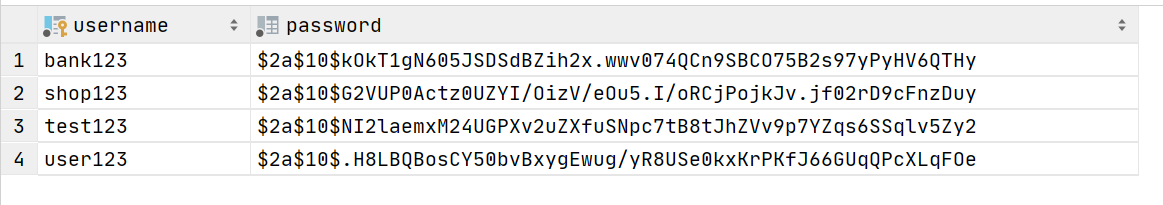
\includegraphics[width=\textwidth]{Clipboard_2021-01-01-10-56-30.png}

\subsection{登录页面}

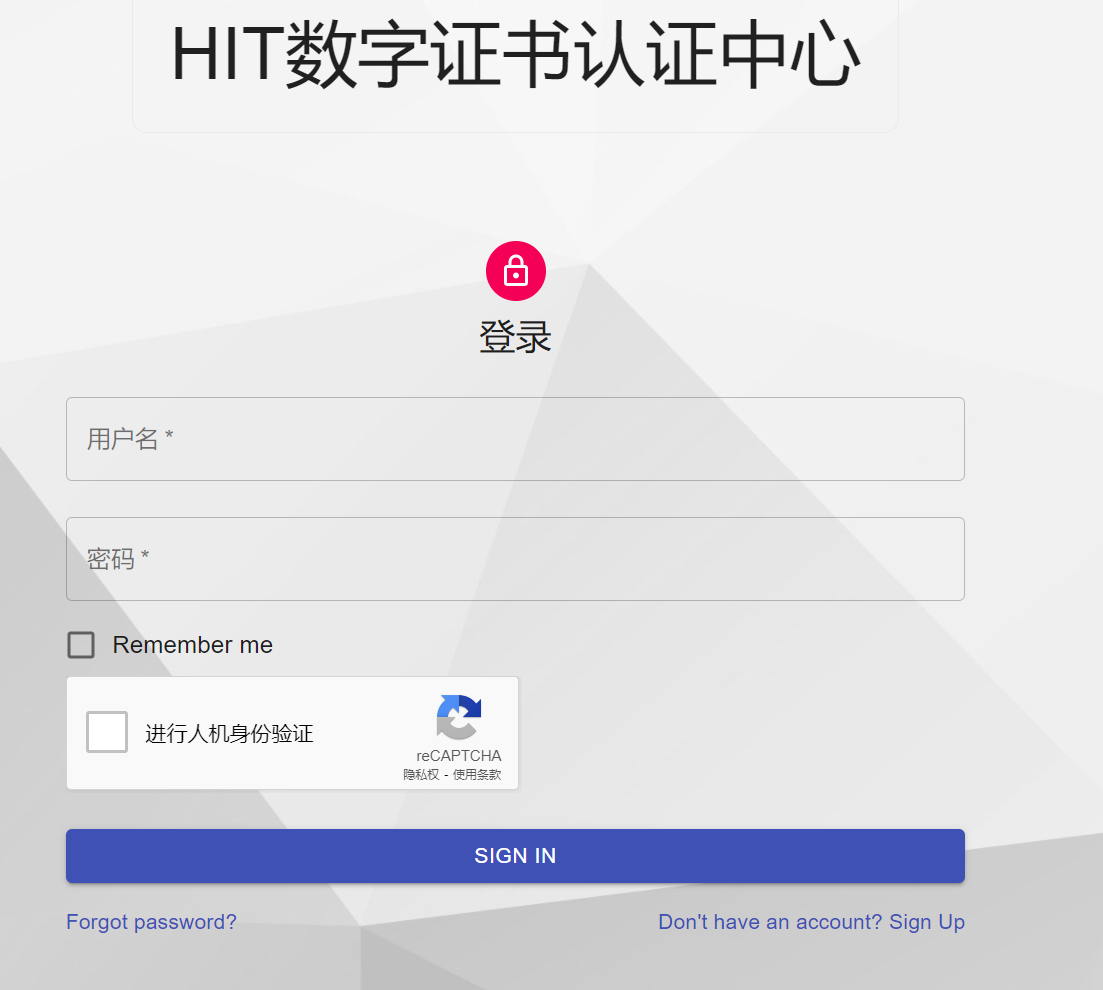
\includegraphics[width=0.7\textwidth]{login_page.png}

用户登录需要输入用户名和密码,需要满足以下几个条件(和用户注册一样):
\begin{itemize}
    \item 用户名必须为字母、数字、下划线、减号的组合,长度为6~16位
    \item 密码至少包括数字和字母,长度至少为6位,至多20位。
\end{itemize}
用户登录需要输入用户名、密码,并通过人机身份验证。后台将从数据库中找到用户名对应的密码,对用户输入的密码用bcrypt哈希后与数据库中的密码比对,如果相同,则登陆成功。\\

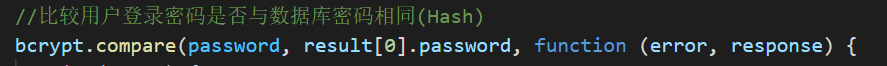
\includegraphics[width=\textwidth]{Clipboard_2021-01-01-11-00-35.png}

\subsection{验证证书页面}

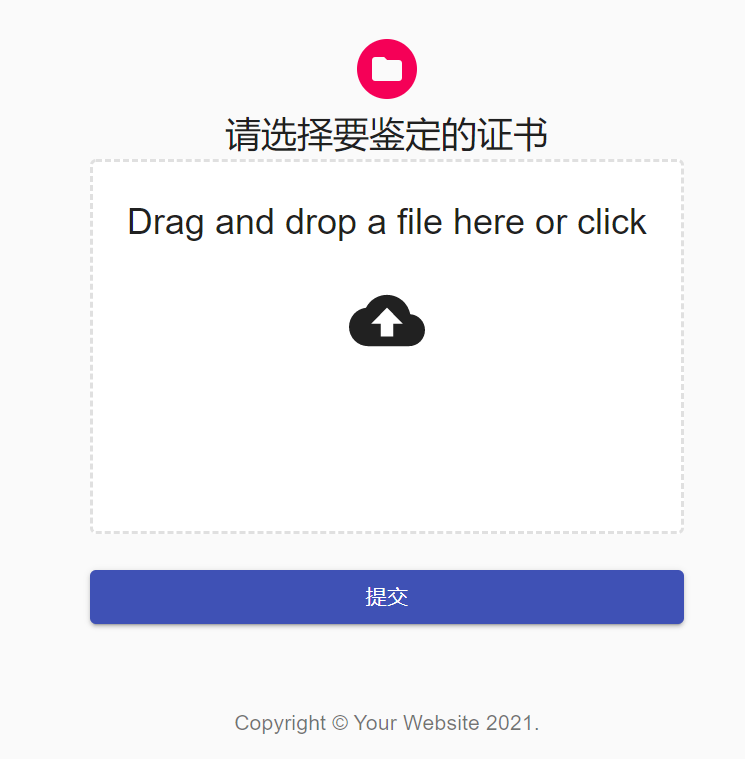
\includegraphics[width=0.5\textwidth]{Clipboard_2021-01-01-11-09-06.png}

用户可以点击上传证书文件(pem格式),点击提交,后端验证证书,如果证书未过期且由本CA签发就会提示证书正确,否则警告证书错误\\


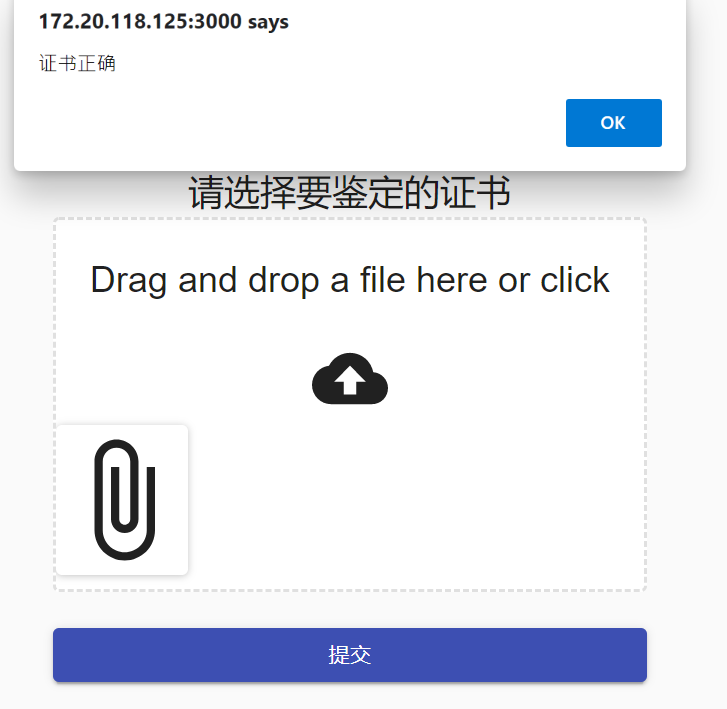
\includegraphics[width=0.5\textwidth]{Clipboard_2021-01-01-11-15-06.png}


\subsection{个人页面}

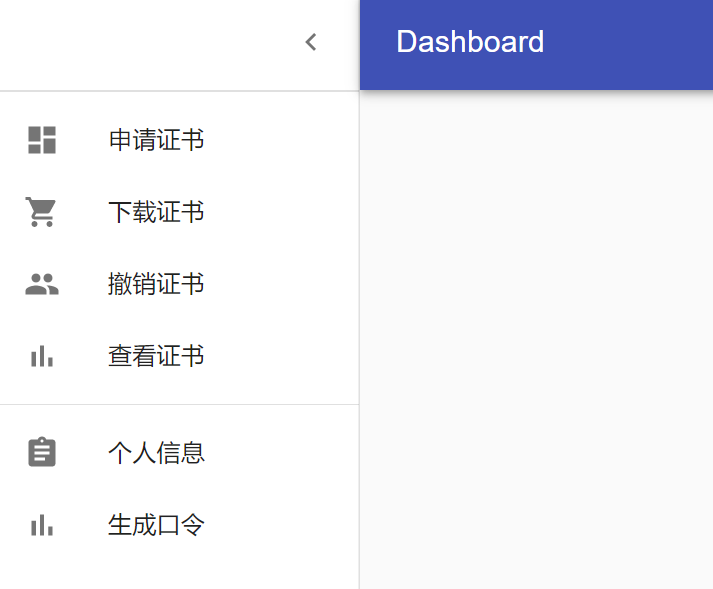
\includegraphics[width=0.5\textwidth]{Clipboard_2021-01-01-11-18-23.png}

只有用户登录后才能进入对应的个人页面,未登录用户选择进入个人页面会直接跳转到登录页面。

进入个人页面后,可以选择相应的功能页面,主操作面板中一共包括6个功能:
\begin{itemize}
    \item 申请证书
    \item 下载证书
    \item 撤销证书
    \item 查看证书
    \item 个人信息(输入口令可以查看私钥)
    \item 生成口令
\end{itemize}



\subsection{申请证书}

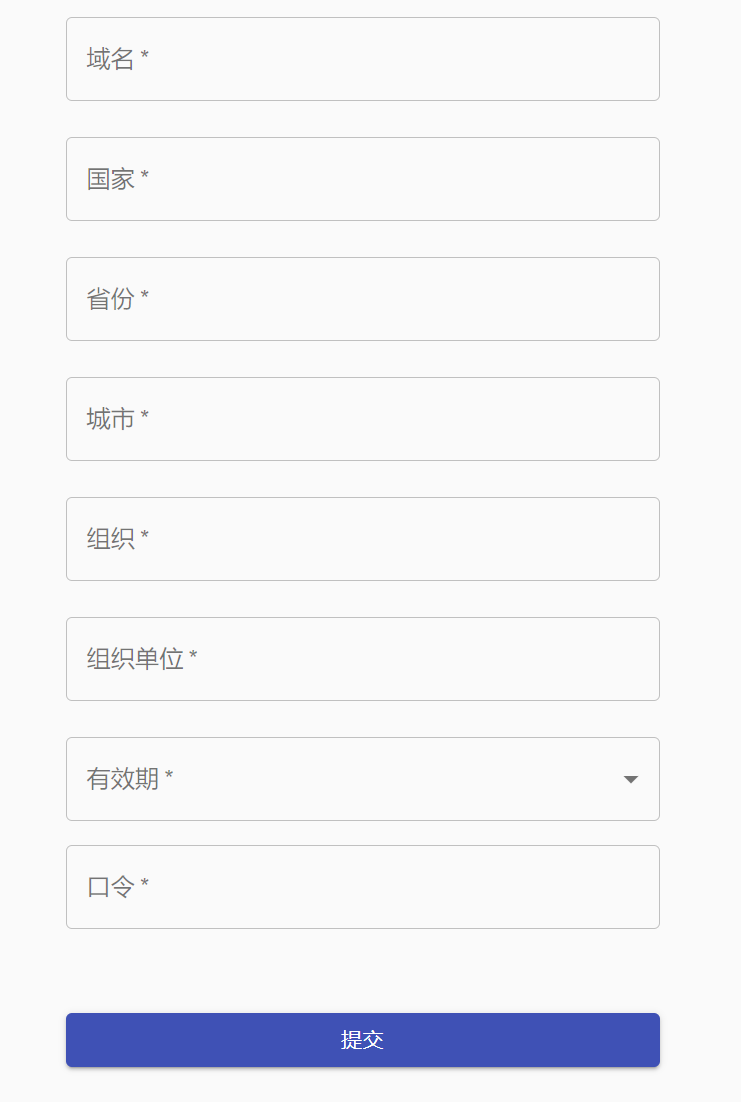
\includegraphics[width=0.5\textwidth]{Clipboard_2021-01-01-11-38-18.png}

申请证书页面包括一个container,其中有用户申请证书需要提交的表单。该表单包括:
\begin{itemize}
    \item 域名
    \item 国家
    \item 省份
    \item 城市
    \item 组织
    \item 组织单位
    \item 有效期(1年/2年/3年)
    \item 口令
\end{itemize}


其中域名即是申请的网站网址,有效期只能三选一,口令用于对私钥加密(可以从生成口令页面中随机生成)


\subsection{下载证书}
用户输入想要下载的证书序列号,点击提交按钮,如果该证书在数据库中就会将证书下载到本地

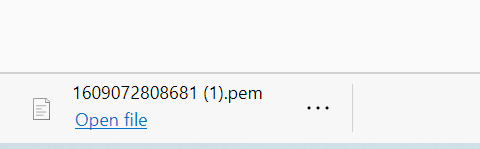
\includegraphics[width=\textwidth]{Clipboard_2021-01-02-14-52-52.png}

点击查看:

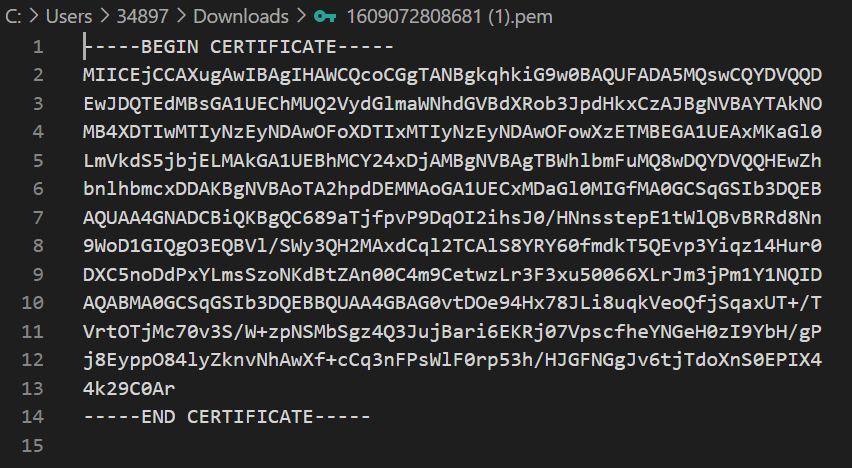
\includegraphics[width=\textwidth]{Clipboard_2021-01-02-14-53-25.png}
\subsection{撤销证书}
用户输入要撤销的证书序列号和用户密码,如果该证书为用户申请并且密码正确,后台验证就可以成功撤销该证书。

其实大型公证CA系统的证书的申请和撤销都是比较严谨的工作,通常需要多方核实,并且在一到三个工作日内给出证书的申请和撤销反馈。本次实验中,对于证书的申请没有加权限(任何登录用户都能申请证书),证书的撤销也只加了登录密码的权限限定(允许用户撤销自己申请的证书)。
\subsection{查看证书}

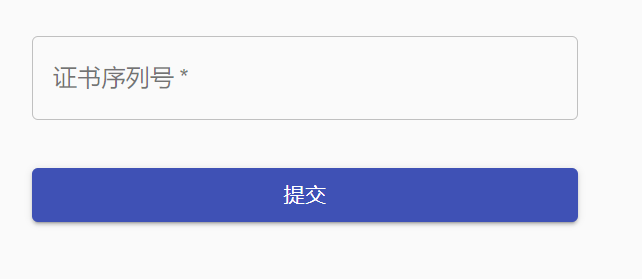
\includegraphics[width=0.5\textwidth]{Clipboard_2021-01-01-15-09-41.png}

用户输入要查看的证书序列号,如果数据库中有该证书,就可以查看到相应证书的信息

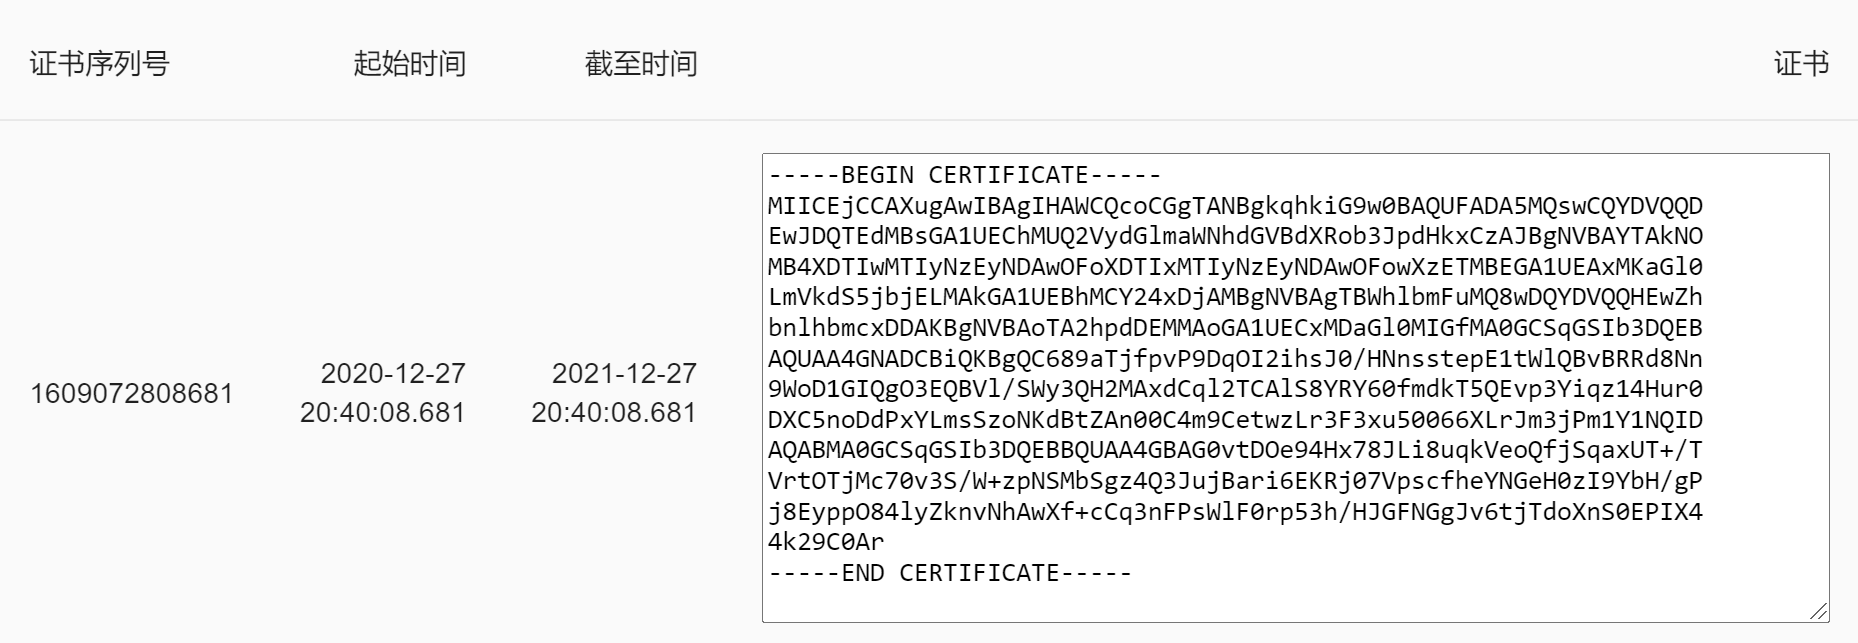
\includegraphics[width=\textwidth]{Clipboard_2021-01-01-15-11-13.png}
\subsection{个人信息}

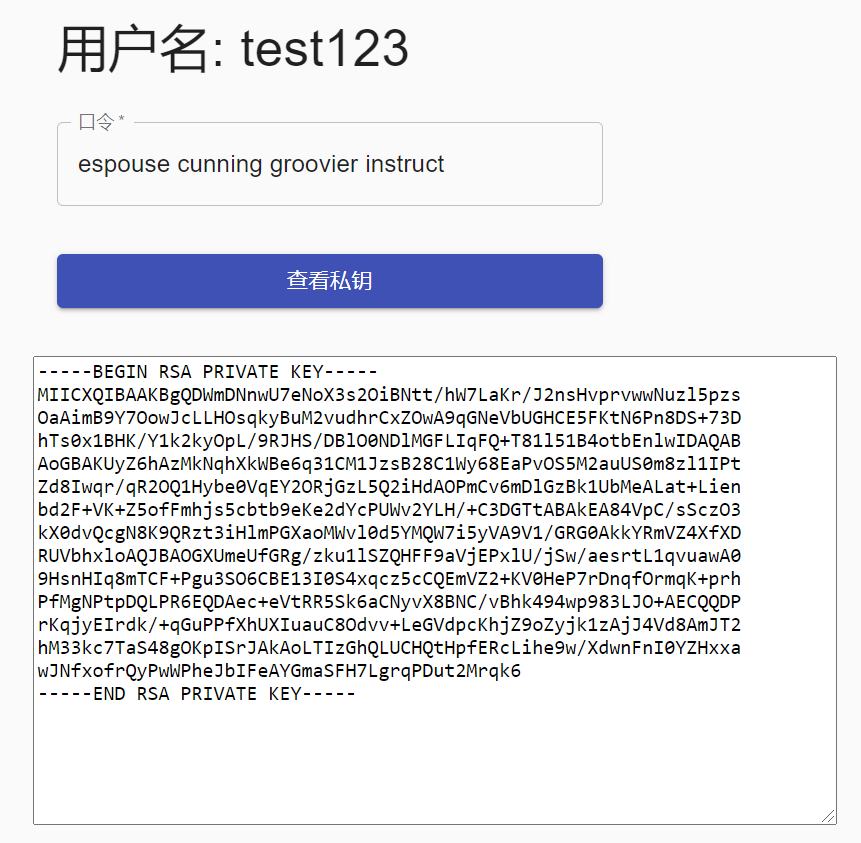
\includegraphics[width=0.7\textwidth]{Clipboard_2021-01-01-15-14-26.png}

用户可以查看当前登录用户名,并且输入申请证书时的口令就可以查看对应私钥
\subsection{生成口令}

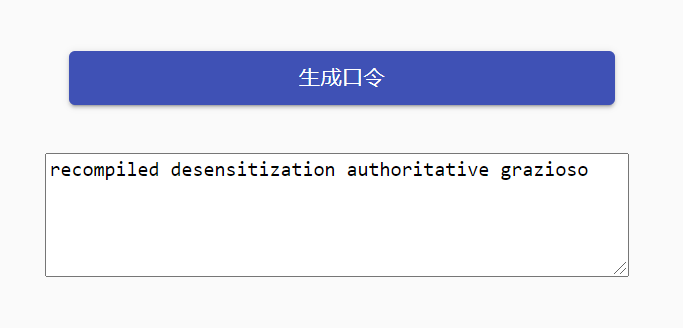
\includegraphics[width=0.7\textwidth]{Clipboard_2021-01-01-15-20-14.png}

每次点击生成口令就可以随机生成一个由4或5个英语单词组成的口令(passphrase),由于口令由英语单词组成,因此相较复杂无规则的口令更容易记忆,同时其安全性甚至更好

安全性分析:从65536个单词的列表中随机选取单词,每个单词的熵值是16bit,因此5个单词的熵值就是80bit,作为口令很难依靠穷举破解(假设敌手每秒尝试1,000,000,000,000次,尝试一半的密钥空间成功破解,其需要的时间大约是1年)
\section{实现与测试}
\subsection{数字证书}
X.509是密码学里公钥证书的格式标准。X.509证书已应用在包括TLS/SSL在内的众多网络协议里,同时它也用在很多非在线应用场景里,比如电子签名服务。X.509证书里含有公钥、身份信息(比如网络主机名,组织的名称或个体名称等)和签名信息(可以是证书签发机构CA的签名,也可以是自签名)。对于一份经由可信的证书签发机构签名或者可以通过其它方式验证的证书,证书的拥有者就可以用证书及相应的私钥来创建安全的通信,对文档进行数字签名。

证书组成结构标准用ASN.1(一种标准的语言)来进行描述,X.509 v3 数字证书结构如下:
\begin{itemize}
    \item 证书 \begin{itemize}
              \item 版本号
              \item 序列号
              \item 签名算法
              \item 颁发者
              \item 证书有效期 \begin{itemize}
                        \item 此日期前无效
                        \item 此日期后无效
                    \end{itemize}
              \item 主题
              \item 主题公钥信息 \begin{itemize}
                        \item 公钥算法
                        \item 主题公钥
                    \end{itemize}
              \item 颁发者唯一身份信息(可选项)
              \item 主题唯一身份信息(可选项)
              \item 扩展信息(可选项)\begin{itemize}
                        \item \ldots
                    \end{itemize}
          \end{itemize}
    \item 证书签名算法
    \item 数字签名
\end{itemize}
数字证书广泛应用在https等网络协议上,我们访问学校官网https://www.hit.edu.cn/,查看网站的证书\\

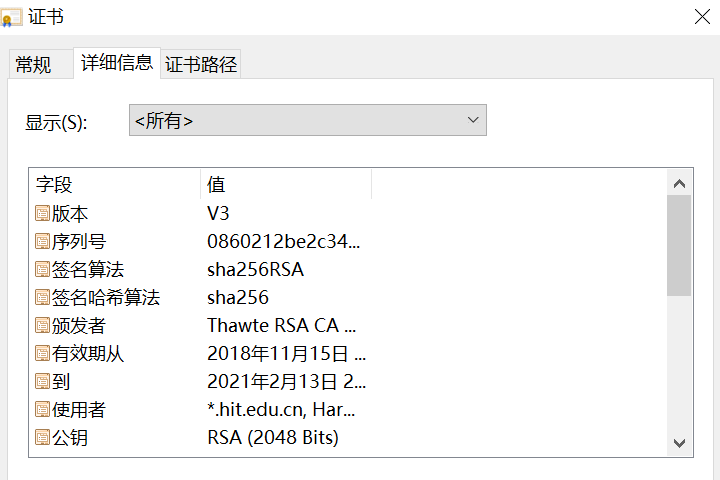
\includegraphics[width=0.7\textwidth]{Clipboard_2021-01-01-16-15-49.png}

我们可以看到版本号、序列号、签名算法等证书信息

参考X.509证书结构,本实验设计实现根证书,将根证书导入到证书列表查看其信息\\

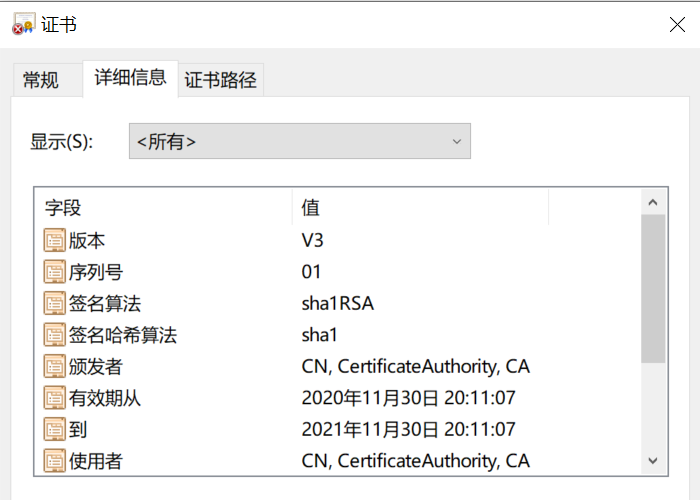
\includegraphics[width=0.7\textwidth]{Clipboard_2021-01-01-16-32-53.png}


本实验需要用户输入域名、国家、省份、城市、组织、组织单位、有效期(1年/2年/3年),然后生成相应的证书。

我们可以将根证书签名的用户证书同样导入到证书列表查看信息,此处以银行申请的证书为例:\\

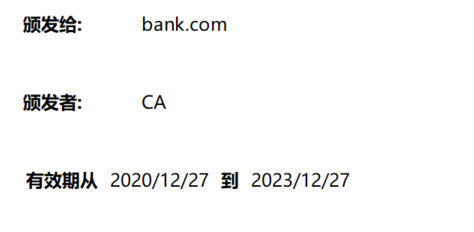
\includegraphics[width=0.5\textwidth]{Clipboard_2021-01-01-16-34-37.png}
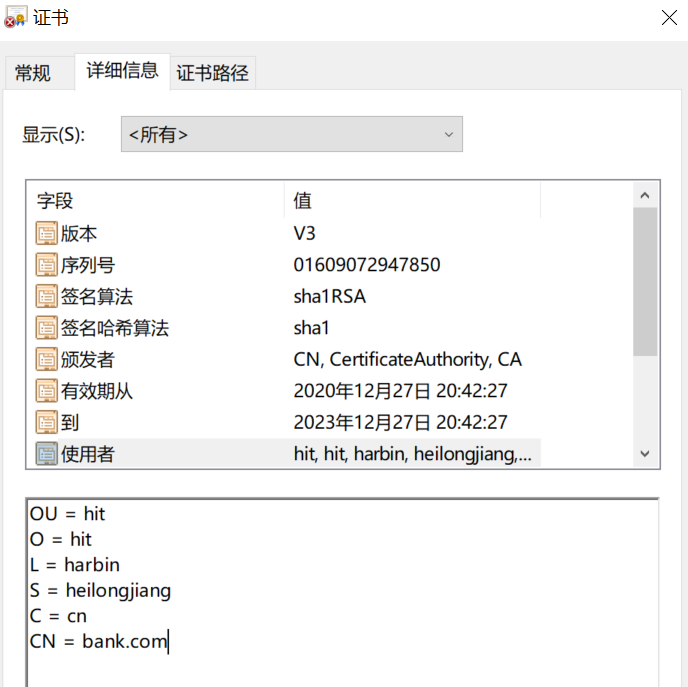
\includegraphics[width=0.5\textwidth]{Clipboard_2021-01-01-16-35-35.png}
\subsection{认证安全}
本CA系统的认证通过jwt(JSON Web Token)实现,当用户成功登录后,后台会签名一个token并存储在localstorage中。对于非公开页面(例如申请证书、撤销证书等个人页面),前端会通过localstorage检查(verify)token,如果不存在或是错误会跳转到登陆页面,这样保证了个人页面只有登录才能查看。最后,本实验设置token时间为1小时,过期后用户需要重新登录。\\

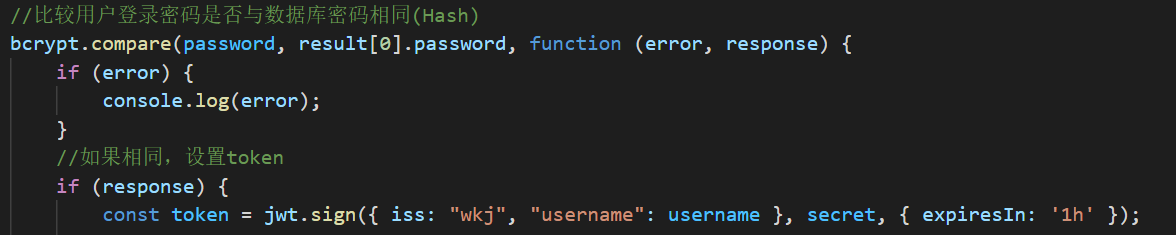
\includegraphics[width=\textwidth]{token.PNG}



\subsection{存储安全}
本CA系统的存储安全只作用在用户密码和证书私钥,由于证书信息是公开的因此没有进行加密。



\begin{itemize}
    \item 对于用户密码,通过bcrypt哈希后存储到数据库中
          \begin{enumerate}
              \item bcrypt是一个由Niels Provos以及David Mazières根据Blowfish加密算法所设计的密码散列函数,于1999年在USENIX中展示。实现中bcrypt会使用一个加盐的流程以防御彩虹表攻击,同时bcrypt还是适应性函数,它可以借由增加迭代之次数来抵御日益增进的电脑运算能力透过暴力法破解。
              \item 由bcrypt加密的文件可在所有支持的操作系统和处理器上进行转移。它的口令必须是8至56个字符,并将在内部被转化为448位的密钥。然而,所提供的所有字符都具有十分重要的意义。密码越强大,您的数据就越安全。
                    相较普通的哈希函数加盐(HMAC)方法,bcrypt一次哈希所需要的时间大大增加,因此敌手依靠穷举破解的办法很难实现。
              \item 例子:在一个普通笔记本电脑,将密码yaaa通过bcrypt哈希需要0.3秒,而用MD5哈希该密码只需要不到一微秒)
          \end{enumerate}




    \item 对于证书私钥,通过用户输入的口令(passphrase)对私钥(message)进行AES加密。由于口令是安全的(难以通过暴力破解),AES加密后的密文也是安全的
\end{itemize}




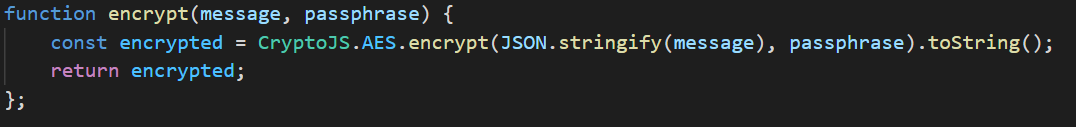
\includegraphics[width=\textwidth]{Clipboard_2021-01-01-17-31-59.png}

\subsection{传输安全}
本小组通过电子信封和双重签名等实现了银行、顾客、电商三方交易信息传输的安全性。借鉴SET协议,银行电商交换证书并通过CA验证证书真伪实现了相互认证(由CA负责为通信双方提供信用担保),如下是验证证书真伪的函数:\\

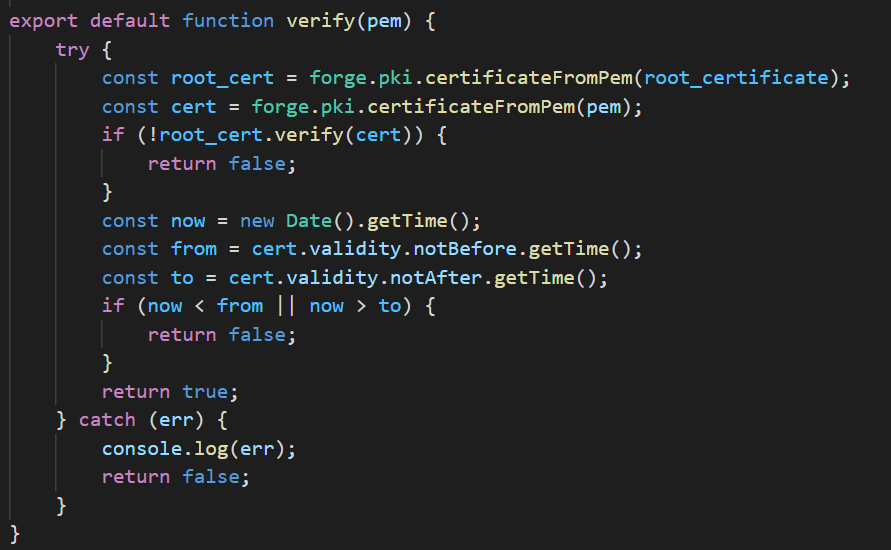
\includegraphics[width=\textwidth]{verify.PNG}

\subsection{注册测试}
我们输入用户名、密码、确认密码,人机验证通过后点击注册按钮就可以成功注册
用户名不合法:\\

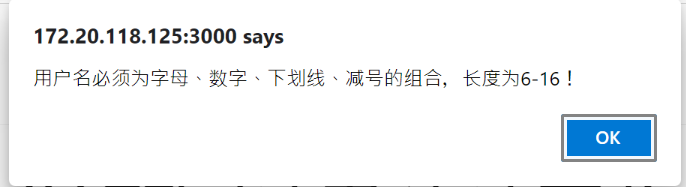
\includegraphics[width=\textwidth]{Clipboard_2021-01-02-14-11-07.png}


密码不合法:\\

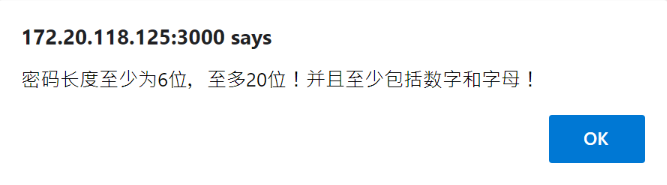
\includegraphics[width=\textwidth]{Clipboard_2021-01-02-14-12-08.png}

两次输入密码不一样:\\

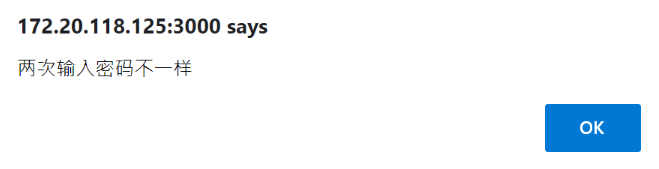
\includegraphics[width=\textwidth]{Clipboard_2021-01-02-14-11-42.png}

未进行人机身份验证:\\

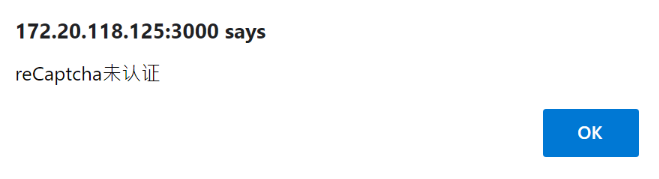
\includegraphics[width=\textwidth]{Clipboard_2021-01-02-14-12-51.png}

注册成功直接跳转到登录界面

\subsection{登录测试}


在登录界面我们输出注册的用户名和密码,人机验证通过后点击登录按钮,后台进行验证,通过后就会进入用户功能页面
用户名不合法:\\

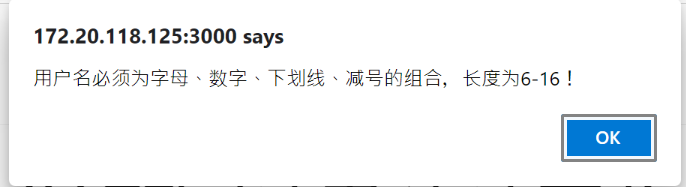
\includegraphics[width=\textwidth]{Clipboard_2021-01-02-14-11-07.png}

密码不合法:\\

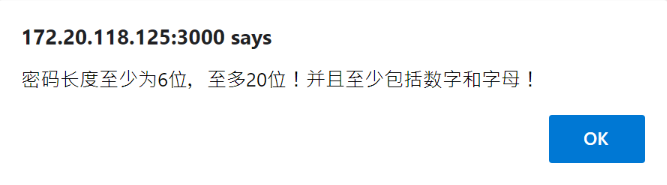
\includegraphics[width=\textwidth]{Clipboard_2021-01-02-14-12-08.png}

未进行人机身份验证:\\

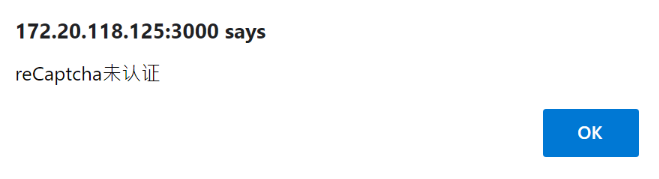
\includegraphics[width=\textwidth]{Clipboard_2021-01-02-14-12-51.png}


用户名/密码错误:当用户的用户名或密码输入错误时,不应该显式地指出到底是用户名错误还是密码错误,防止攻击者对用户名或密码针对性的攻击。\\
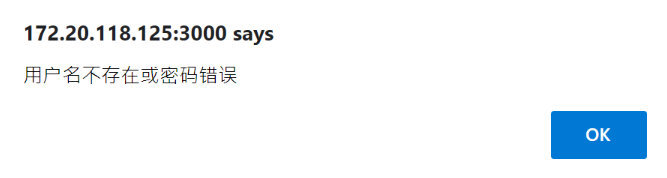
\includegraphics[width=\textwidth]{Clipboard_2021-01-02-14-41-45.png}



登录成功后跳转到用户界面
\subsection{申请证书测试}

用户输入证书相关信息和私钥口令,点击提交按钮,申请的证书就会下载到本地 \\

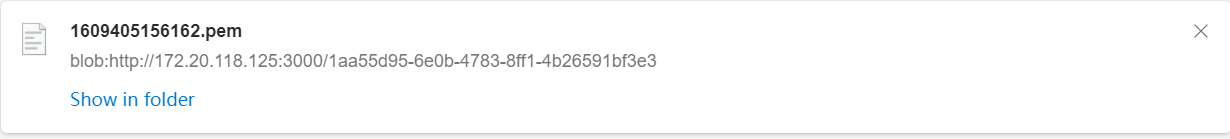
\includegraphics[width=\textwidth]{Clipboard_2021-01-02-14-48-51.png}

点击查看:\\

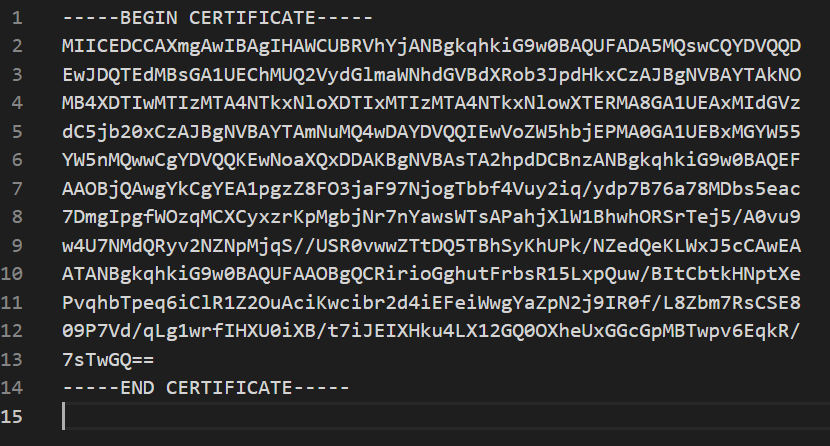
\includegraphics[width=\textwidth]{Clipboard_2021-01-02-14-47-56.png}


\subsection{验证码}
验证码的作用是为了给恶意破解密码、反复自动提交表单攻击造成麻烦。本CA系统中要求用户登录/注册时进行人机身份验证。

本实验采用的验证码是Google的reCAPTCHA,系统会对用户在网站上的动作进行评分,如果正常点击进行人机身份验证即可通过\\

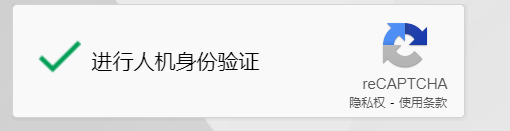
\includegraphics[width=0.5\textwidth]{Clipboard_2021-01-01-16-51-30.png}


否则系统判别异常,就会要求用户选择包括某一物体的所有图块,正确选择后才可通过

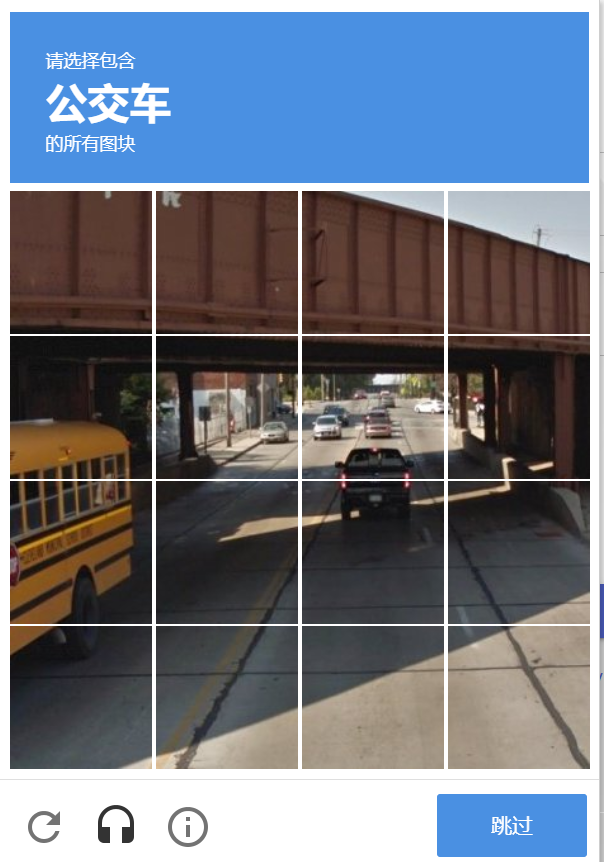
\includegraphics[width=0.5\textwidth]{Clipboard_2021-01-01-16-53-28.png}
\subsection{口令}
区别于密码,口令应该容易被人记忆,但难以被敌手破解。本实验要求用户在申请证书时输入口令用来加密私钥。之后用户可以通过输入口令得到私钥,CA只保存加密的私钥而不保存口令,其他任何人在不知道口令的情况下即使破解数据库也没用(数据库中的私钥用口令AES加密)。

本实验采用的是由英语单词构成的口令,英语单词在65536个单词的列表中随机选取。这样用户只需要记忆几个英语单词即可,而靠蛮力破解口令非常困难。
\subsection{密码隐藏显示}
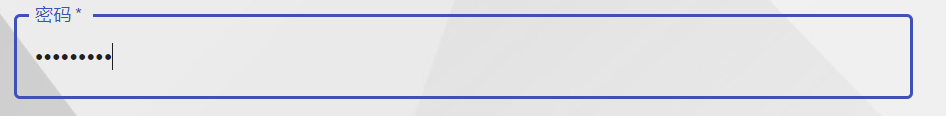
\includegraphics[width=0.8\textwidth]{Clipboard_2021-01-01-17-36-14.png}

本实验登录、注册页面密码默认隐藏,可以避免偷窥攻击。

\section{结束语}
经过了八周的密码学实验实践,从最初基本的构思到最终各种功能的实现,实现了一个具有申请、撤销、下载、查询等基本功能的CA认证系统

通过这次实验,我学习了前端框架react,掌握了mysql数据库的各种基本操作,了解到了传输安全、存储安全等概念,通过自行设计数字证书对数字证书有了更深的理解

最后,我和我的队友们三个人合作为了将各自的程序交互起来,在开发过程中团队积极相互沟通,解决了很多困难,我也理解到了团队合作的重要性


\section{参考文献}
\begin{itemize}
    \item X.509-维基百科 [https://en.wikipedia.org/wiki/X.509]
    \item Optimizing Performance - React [https://reactjs.org/docs/optimizing-performance.html]
    \item reCAPTCHA-维基百科 [https://en.wikipedia.org/wiki/ReCAPTCHA]
    \item bcrypt-维基百科 [https://zh.wikipedia.org/zh-cn/bcrypt]
    \item How To Safely Store A Password [https://codahale.com/how-to-safely-store-a-password]
\end{itemize}


\end{document}